\chapter{Deep Learning}

\section{Was ist Deep Learning?}

\section{Problemstellung}

Gegeben sei ein Kamerabild $I_D$, welches von einem Duckiebot $D$ aufgenommen wurde. Das Bild $I_D$ wird einem Posenschätzer $E$ zur Verfügung gestellt, welcher dann den Abstand $d_D$ sowie die Orientierung $\Theta_D$ des Duckiebots zur rechten 
Fahrbahnmarkierung ermitteln soll. Der Posenschätzer ist hierbei ein künstliches neuronales Netz, um die oben genannte Problemstellung lösen zu können. Als Lernverfahren wird überwachtes Lernen eingesetzt.

\section{Datensatzerstellung}

Damit der Posenschätzer seine Aufgabe erfüllen kann, muss zunächst ein Datensatz erstellt werden, damit dieser trainiert werden kann. Der Datensatz besteht dabei aus einem Trainingsdatensatz, einem Validierungsdatensatz sowie aus einem Testdatensatz. \\

Der Trainingsdatensatz ist ein Beispieldatensatz der für das Lernen der Muster und Zusammenhänge in den Daten verwendet wird. Das Modell des neuronalen Netz nutzt also diese Daten um zu lernen. \cite{datasolut} \\

Der Validierungsdatensatz ist ebenso ein Beispieldatensatz, welcher für die Abstimmung der Hyperparameter des Modells des neuronalen Netzes verwendet wird. Dadurch wird das sognenannte \glqq Overfitting\grqq{} (Überanpassung) des Modells auf die Trainingsdaten verhindert. \cite{datasolut} \\

Der Testdatensatz ist ebenfalls ein Beispieldatensatz, jedoch sind die Daten von den Trainingsdaten unabhängig. Die Testdaten werden beim Training des neuronalen Netzes nicht benutzt, sondern dienen zur abschließenden Verifikation des Modells. Dadurch kann die Qualität des Modell erfasst werden, damit man eine Aussage über die Leistungsfähigkeit des neuronalen Netzes treffen kann. \cite{datasolut} \\

Die oben genannten Datensätze wurden mit Hilfe des Duckietownsimulators automatisiert erstellt. Ein Eintrage eines Datensatzes besteht hierbei aus dem Kamerabild $I_D$, welches mit dem dazugehörigen Abstandswert $d_D$ sowie Orientierungswert $\Theta_D$ beschriftet wurde. Der Trainingsdatensatz besteht hierbei aus X Einträgen, der Validierungsdatensatz aus X Einträgen und der Testdatensatz aus X Einträgen. Die Abbildung \ref{fig:data_entry_example} zeigt einige beispielhafte Einträge eines Datensatzes.

\begin{figure}[H]
	\centering
	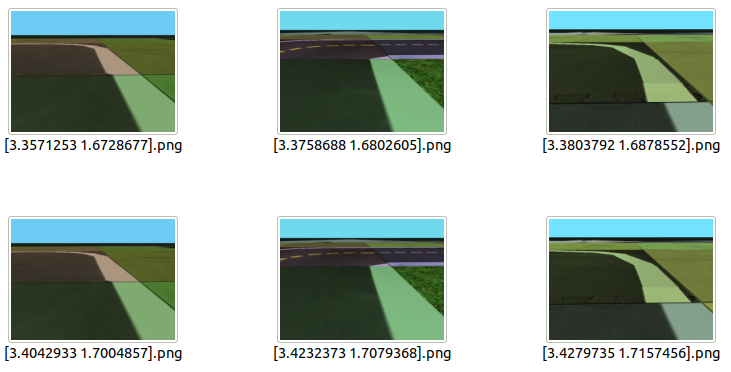
\includegraphics[width=0.8\textwidth]{kapitel3/images/dataset_entries_example.png}
	\caption{Beispielhafte Einträge eines Datensatzes}
	\label{fig:data_entry_example}
\end{figure}


\section{Netzwerkarchitektur}



